\documentclass[11pt]{article}
\usepackage{fullpage}
\usepackage{graphicx}
\graphicspath{ {./images/} }

\title{CS63 Fall 2020\\Lab 6: Convolutional Neural Networks}
\author{Ankur Malik, Ibrahem Hassouna}
\date{March 31, 2022}

\begin{document}
\begin{center}

\maketitle

\section{Data Set}

% TODO Describe the data set.
% TODO Explain the format of the data.
In this model, we are using the Fashion MNIST. Fashion MNIST is a data set of images; it contains a training set of 60,000 examples and a test set of 10,000 examples.
Each example is a 28x28 image, associated with a label from 10 classes.
Each pixel has an integer value associated with it, indicating the lightness or darkness of that pixel, with higher numbers meaning darker.
Fashion-MNIST is very similar to the MNIST data set (handwritten digits) and they are both used to benchmark machine learning algorithms.
They both share the same image size and structure of training and testing splits.
\linebreak
Each example is mapped to one of the following labels:
\begin{itemize}
  \item 0 T-shirt/top
  \item 1 Trouser
  \item 2 Pullover
  \item 3 Dress
  \item 4 Coat
  \item 5 Sandal
  \item 6 Shirt
  \item 7 Sneaker
  \item 8 Bag
  \item 9 Ankle boot
\end{itemize}
\linebreak
After getting the data set, we perform several operations to prepare the data for the model. The first operation is to normalize the input so that it all be within the range [0,1].
The second operation is to convert the output vector into a one-hot vector. A one-hot vector is a vector that has all zeros except one entry that is equal to one,
signaling which label (category) the observation has been classified as.

\section{Network}

% TODO Summarize the network architecture you chose.

% TODO Explain what alternative network architectures you considered,
% and why you ended up with the one you did.

{\bf Baseline model}
\linebreak
We have modified the number of epochs from 5 to 10 in order to allow for more learning to occur (ie. leading to a better model).
When val\_loss has plateaued, this is indicative that further training of the model will not lead to better performance on the validation (test) data set. Thus, training beyond this point will result only in the model learning the training data set better, while not improving or even deteriorating in performance on the test data set. This phenomenon is known as overfitting and is a common pitfall in the study of neural networks.
\linebreak
Let us lay out the construction of the baseline model below:
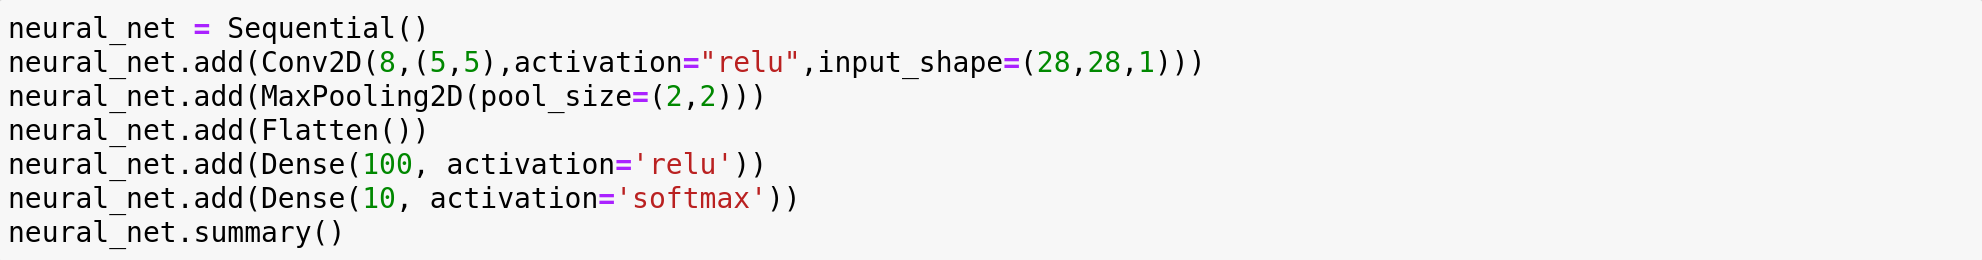
\includegraphics[scale=0.25]{Baseline_construct}
After training the model, we get the following results:
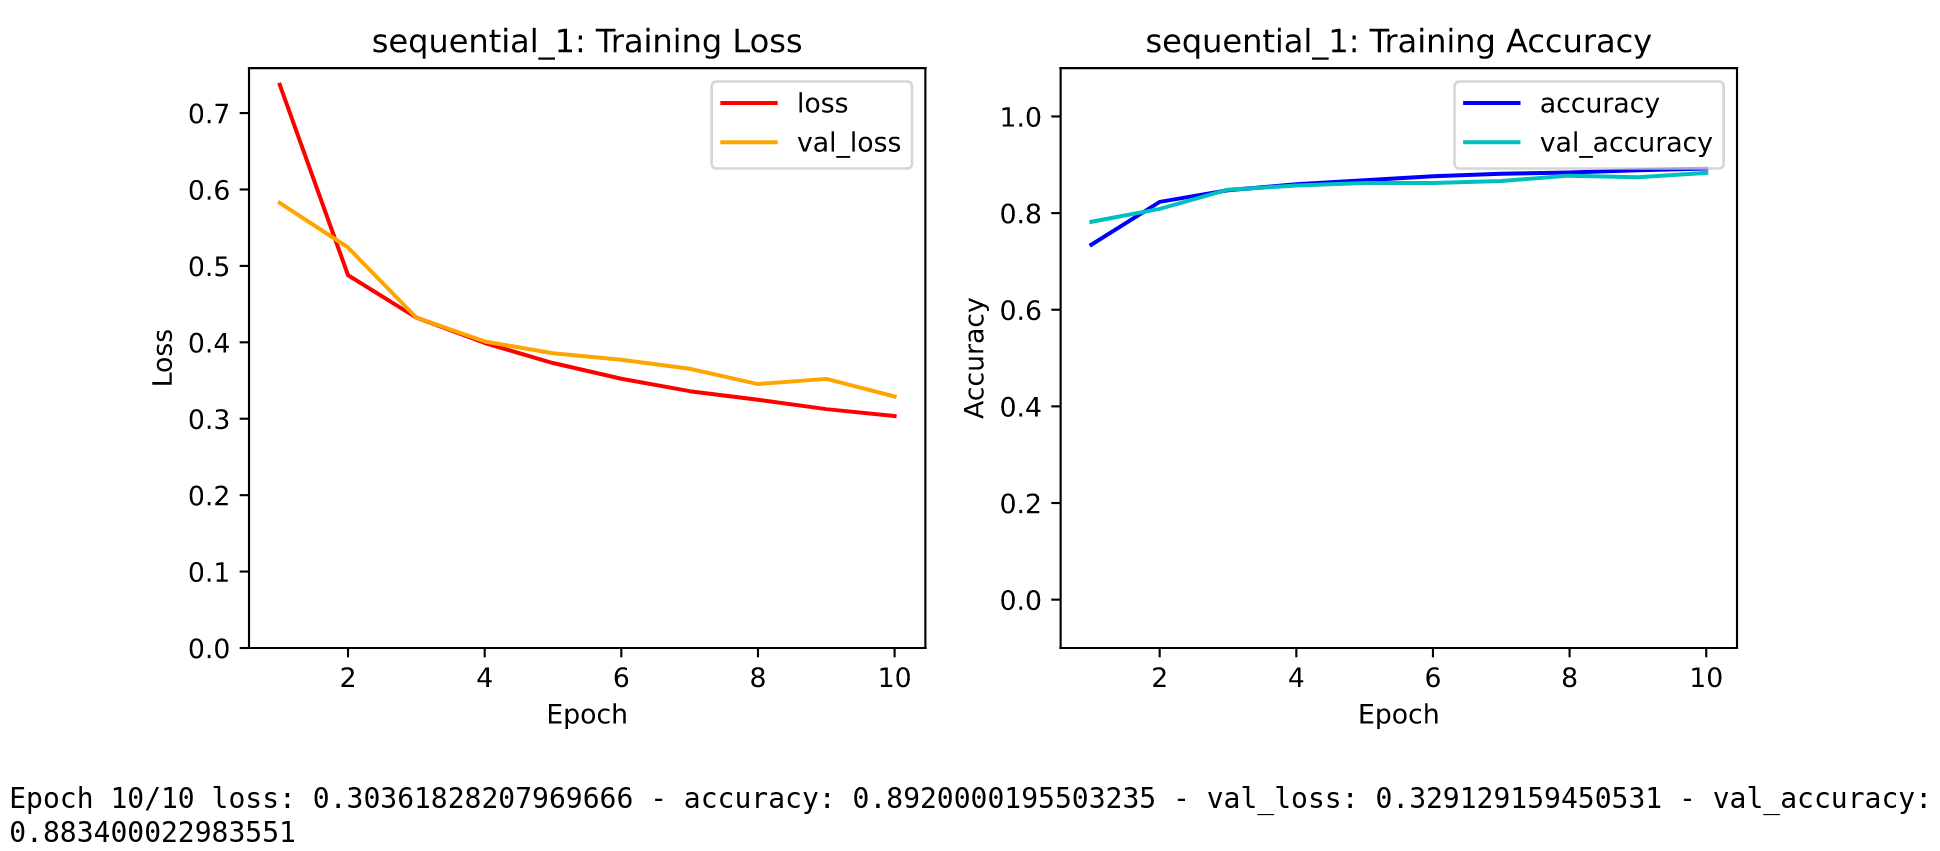
\includegraphics[scale=0.25]{Baseline_train}
The number of incorrectly classified images at this juncture is 1166.

{\bf Changes to baseline model}
\linebreak
We made several alterations and additions to the already provided (baseline) model - these were as follows:
\begin{itemize}
  \item Modification and Addition of Conv2D Layers
  \item Removal of Pooling Layer
  \item Increase Number of Units in First Dense Layer
  \item Addition of Dropout Layer
\end{itemize}
{\bf Modification of existing Conv2D layer; addition of Conv2D layers:}
First, we quadruple the number of units in our first Conv2D layer from 8 to 32. At the same time, we reduce the dimensions of the receptive field to (3,3).
Utilizing a smaller receptive field allows the model to focus on patterns and features that may otherwise be missed at the larger initial dimensions of (5,5).
Additionally, we include two more Conv2D layers immediately following this first Conv2D layer, doubling the number of units consecutively - therefore, layers
of 64 and 128 units respectively. Both layers utilize the same dimensions for the receptive field as the first layer, namely (3,3). The rationale for adding
these layers is to increase the number of trainable parameters, making the model more complex and increasing its ability to generalize to data not seen before
(ie. the test or validation data set).

{\bf Removal of Pooling layer:}
Since we are already incorporating a degree of abstraction through the Conv2D layers above (by having the units analyze multi-pixel areas of the image), it is
not necessarily the case that the inclusion of a pooling layer following these Conv2D layers improves performance, despite the fact that in many instances
these two layers follow each other in a sequential fashion. Indeed, we found that our model's performance improved with the removal of the pooling layer,
which is why it is not part of the construction of our final model.

{\bf Increase Number of Units in First Dense Layer:}
We increased the number of units from 100 to 128. Similar to the rationale for including additional Conv2D layers, packing more units into a dense layer
increases the number of trainable parameters, which can ultimately improve model performance as long as one eye is kept on overfitting, as our goal is
not to optimize performance on the training data set but rather on the test data set to ensure the model is generalizing effectively.

{\bf Addition of Dropout Layer:}
Dropout randomly chooses to drop a percentage of units in the model (ie. set them to 0) in order to prevent overfitting. When a model contains so many (trainable)
parameters, as our model does, overfitting becomes a clear hazard to avoid. 0.2 is a good starting point and we elected to keep the dropout rate to this level.
Since this is a random process, model performance (best benchmarked by val\_loss and val\_accuracy) will differ slightly from iteration to iteration.

{\bf Final Model}
\linebreak
The construction of the final model is below:
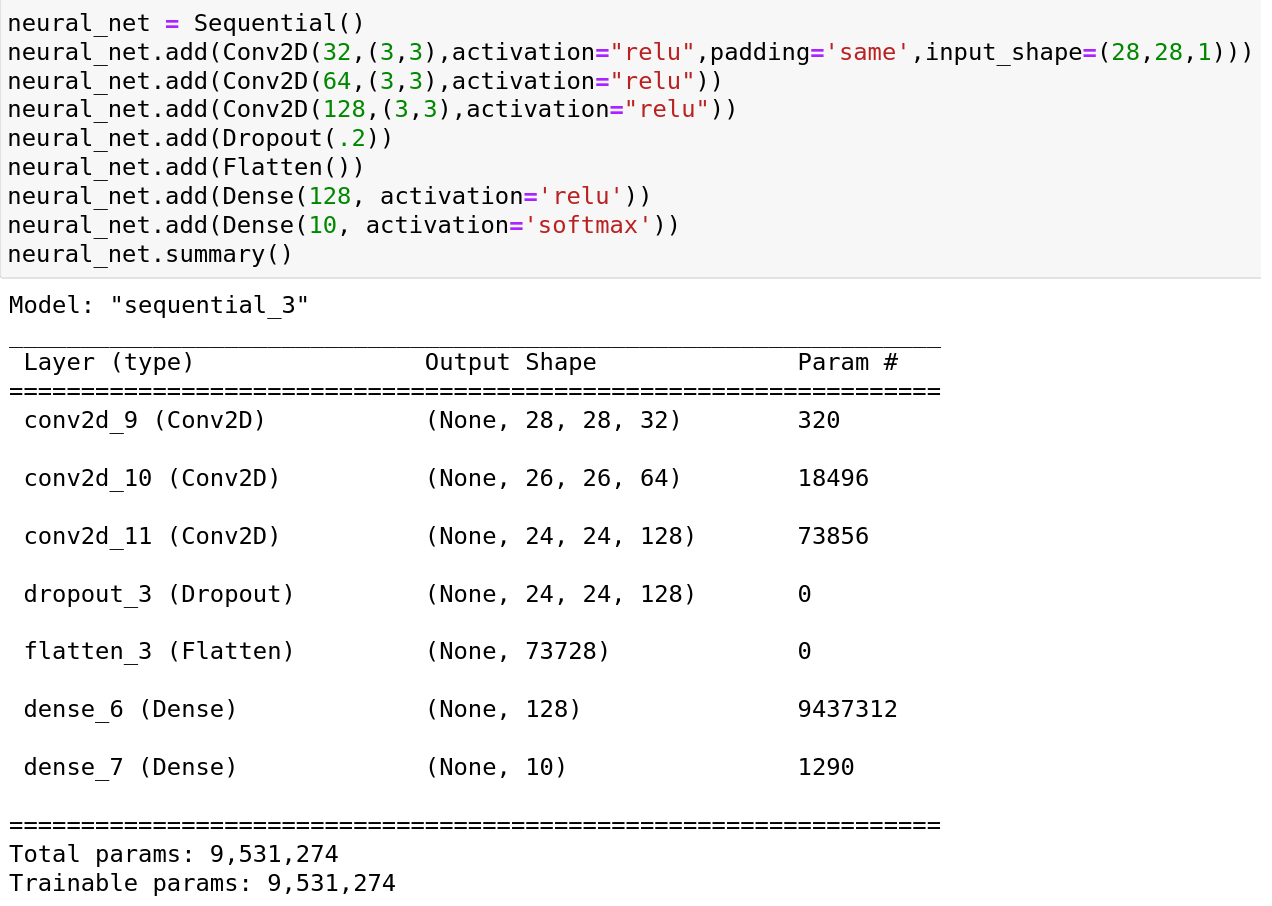
\includegraphics[scale=0.25]{Final_dropout_construct}
\linebreak
After training the model, we get the following results:
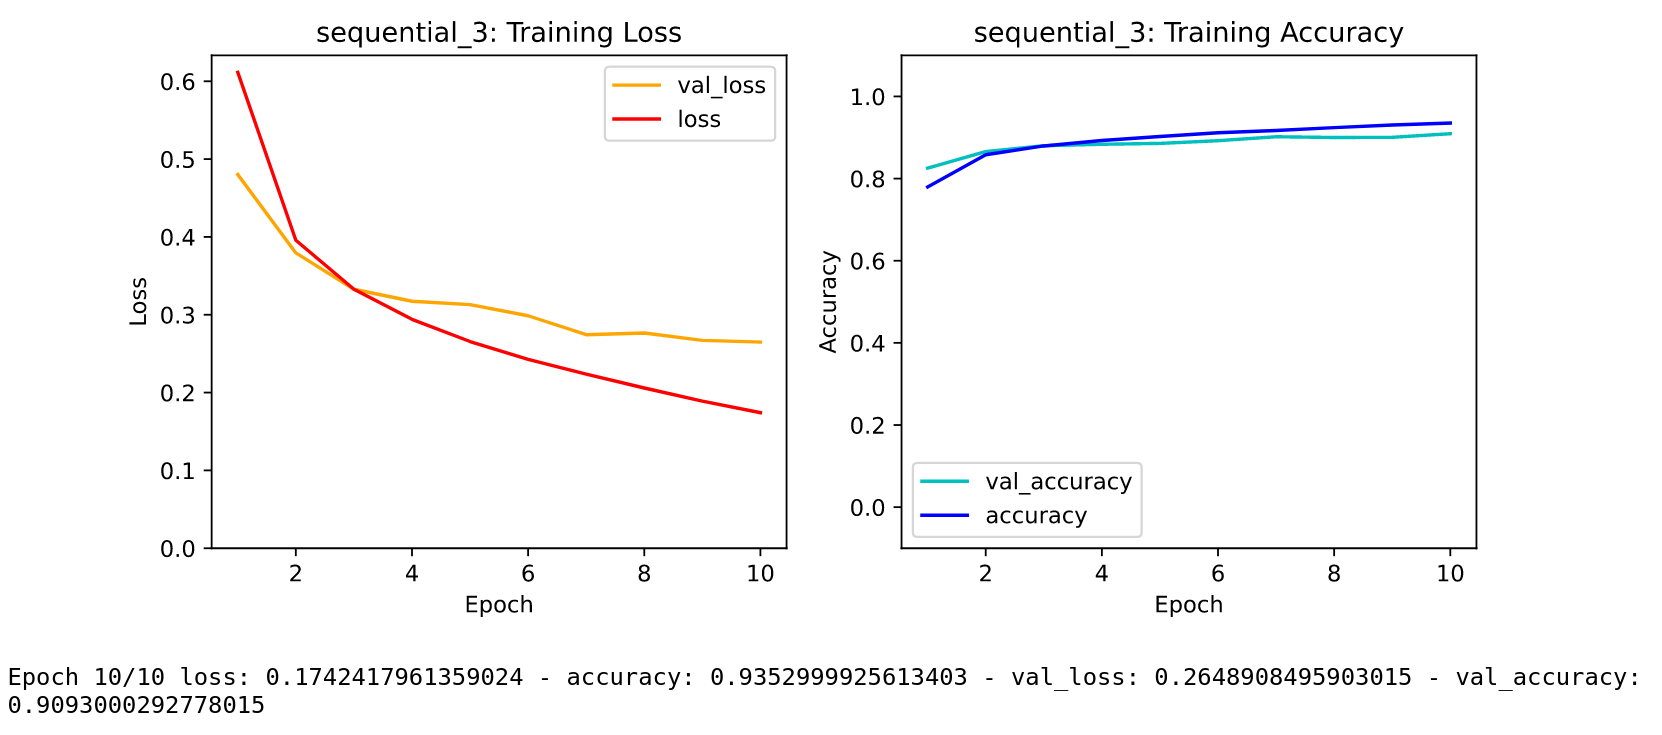
\includegraphics[scale=0.25]{Final_dropout_train}
\linebreak
The number of incorrectly classified images has decreased (not sure exactly what the number is, as we are getting weird errors in the "Examine Results" section and feature maps
all of a sudden!). However, we definitely saw the number going down during our experimentation process!

\section{Evaluation}

% TODO Explain what experiments you did and what metrics you used to
% test the success of your network.

% TODO Show some results of these tests.  Are there patterns in the
% types of images that are successfully classified vs the ones that
% are misclassified?

We tinkered and experimented with several different aspects of the model as documented above. For example, we realized that the removal of the pooling layer (after adding another
Conv2D layer to the model) led to better performance in terms of val\_loss and val\_accuracy, as seen below. Here is the model construction and its corresponding performance
with pooling:
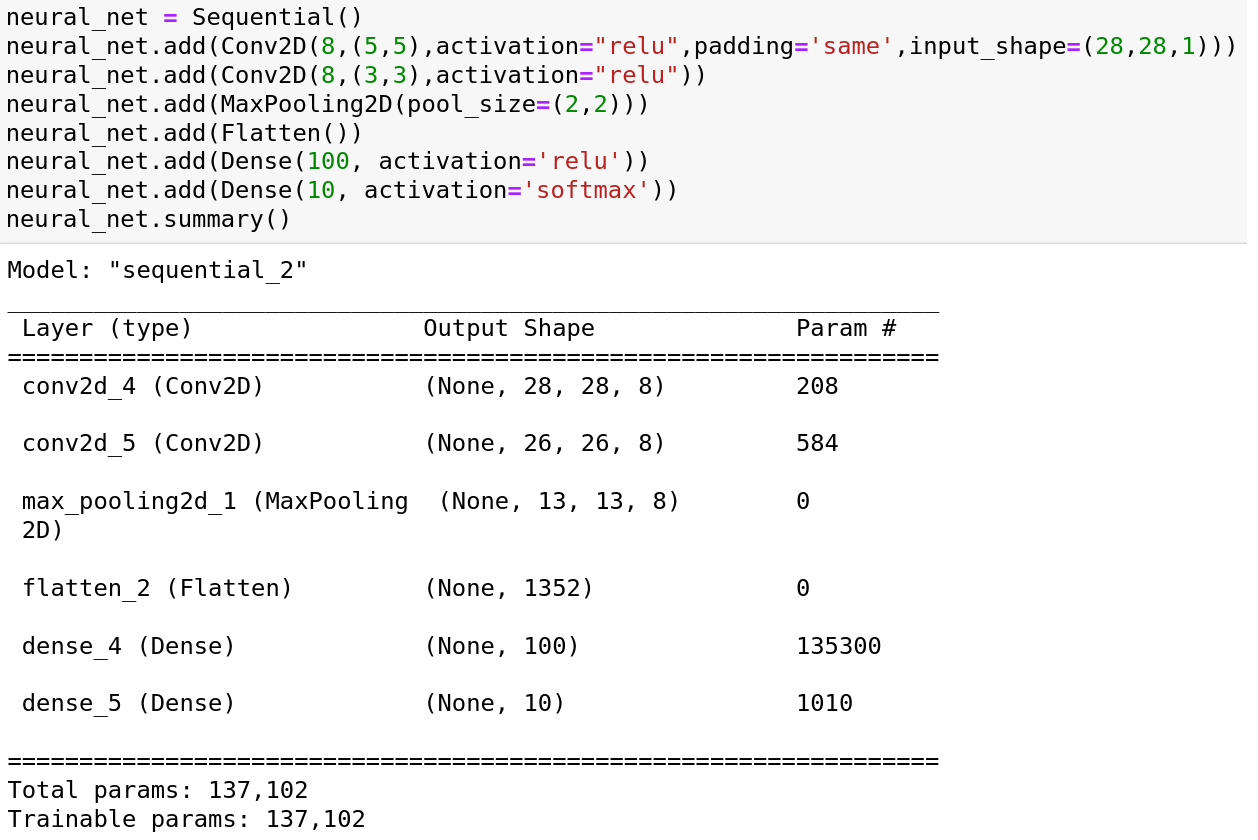
\includegraphics[scale=0.25]{W_pooling_construct}
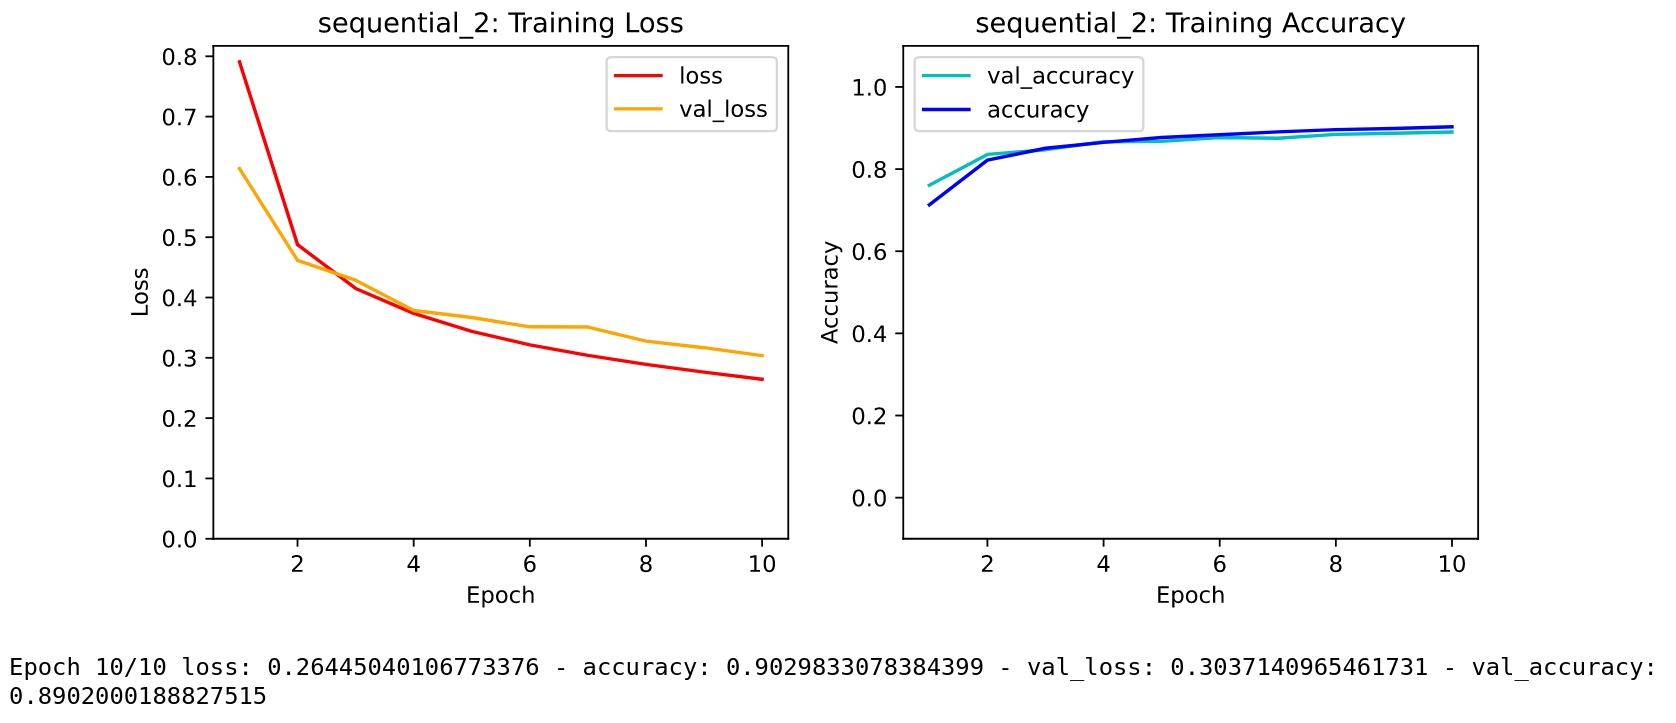
\includegraphics[scale=0.25]{W_pooling_train}
\linebreak
After removing the pooling layer, the model construction and performance is now:
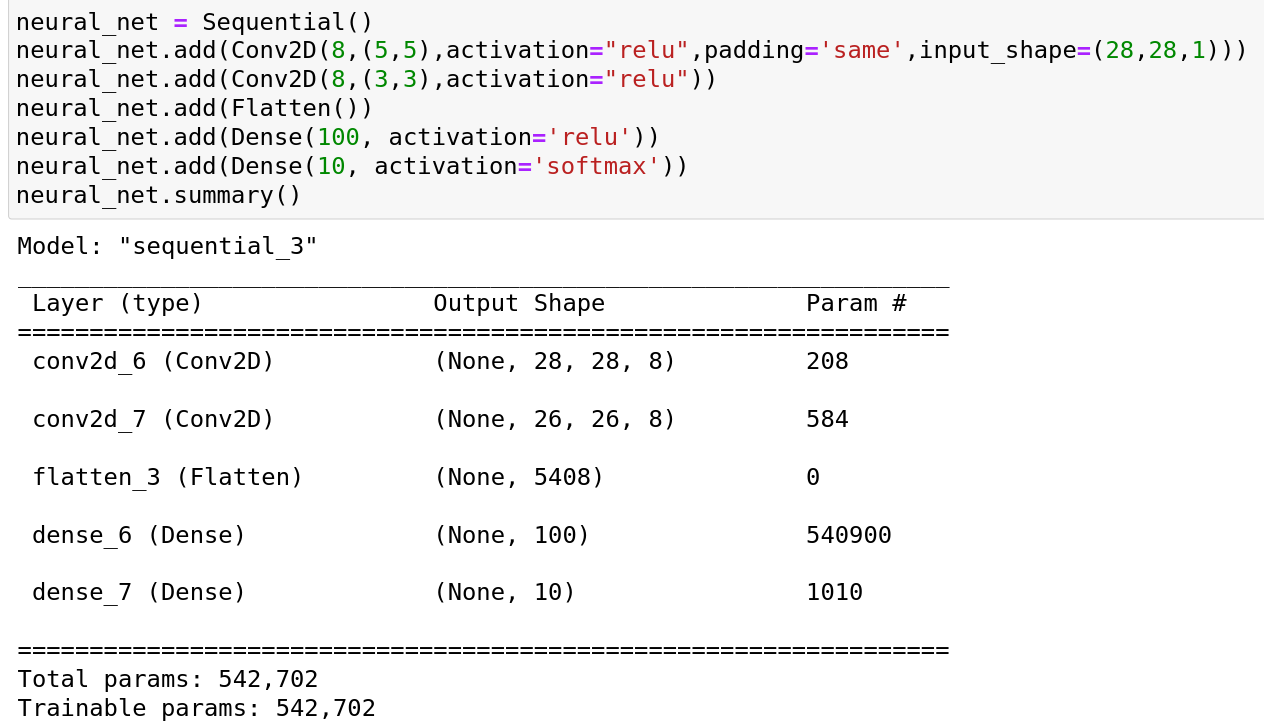
\includegraphics[scale=0.25]{W_o_pooling_construct}
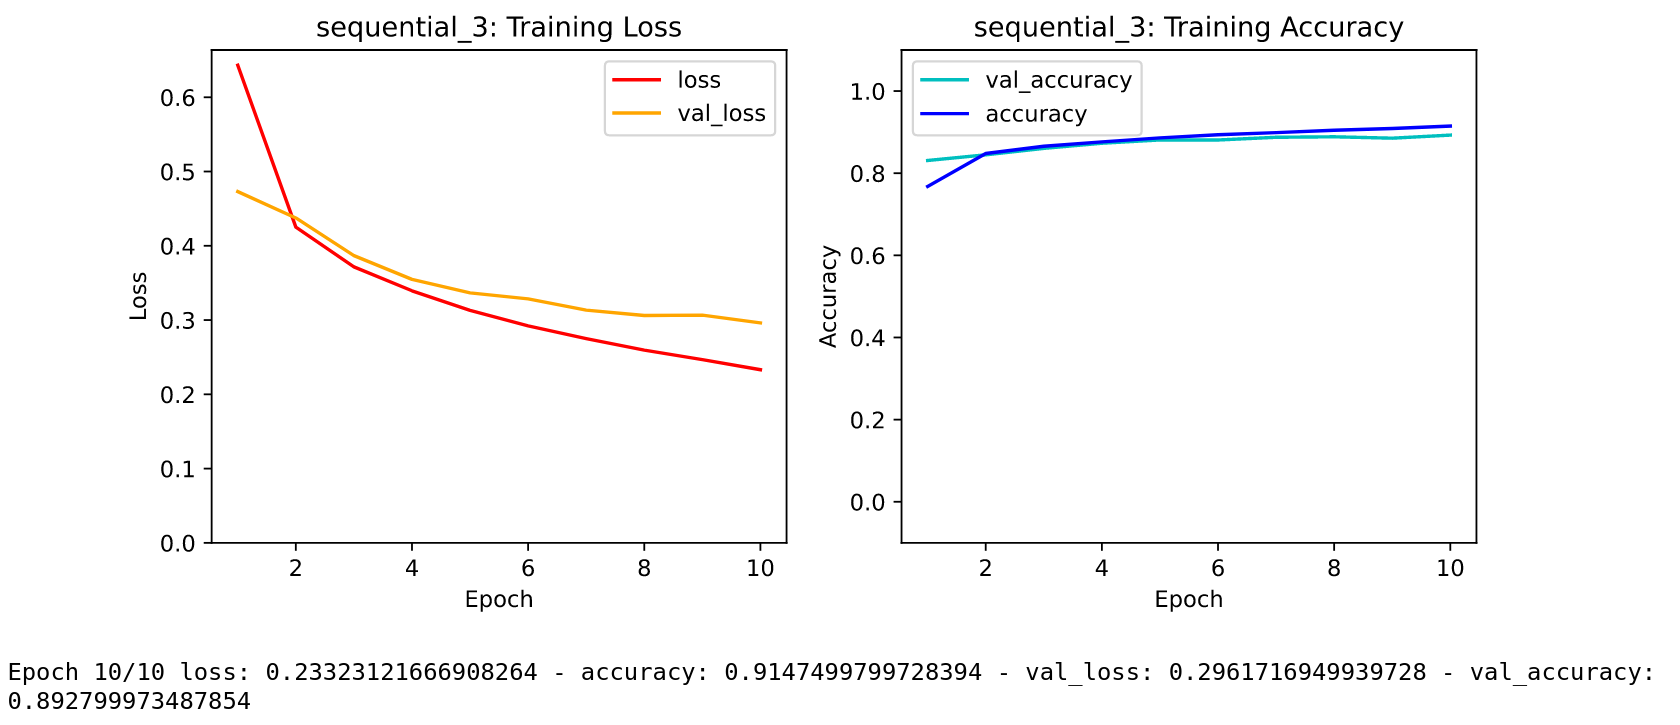
\includegraphics[scale=0.25]{W_o_pooling_train}

\section{Discussion}
% TODO Explain what your network was good at and why.
% TODO Explain what your network was bad at and why.

Ultimately, our network was able to achieve quite high accuracy on the test data set (approx. 90 percent). Minimization of loss on the test data set (loss being the distance between the
true label of an example and the label chosen by the model) was not as successful - we were able to reach a rate of loss of 0.265.

\end{center}
\end{document}
